\chapter{에임}{\label{chap:aim}}
\section{introduction : 에임의 목표와 요소}
에임의 목적은 시선과 크로스헤어, 즉 마우스 움직임의 동기화이다. 즉, 내가 보는 곳으로 에임을 옮기는 것이다. 따라서 에임을 하기 위해서는 우선 눈으로 상대를 인식해야 하며, 마우스를 옮겨 크로스헤어를 상대 위에 가져다두어야 한다. 그리고 마우스를 옮기는 동작은 팔에 달린 수많은 근육과 힘줄이 수행한다. 여기까지의 논의를 바탕으로 에임 연습의 목적은
\begin{enumerate}
    \item 팔과 손목, 손가락의 움직임과 마우스의 움직임 사이의 관계를 익히고
    \item 마우스의 움직임과 크로스헤어의 움직임 사이의 관계를 익혀서
    \item 신체의 움직임과 크로스헤어의 움직임을 연결하는
\end{enumerate}것이라고 할 수 있다.\footnote{마우스의 움직임과 크로스헤어의 움직임 사이에는 1대1대응 및 선형성이 성립하지만, 근육의 움직임과 마우스의 움직임 사이에는 선형성은 보장할 수 없으므로 학습이 필요하다.}
그러므로
에이밍은 시선, 자세, 감도, 관절가동범위, 지지대 등 수많은 요소들이 복합적으로 작용하는 동작이라고 할 수 있다. 에임을 쉽게 맞추기 위한 뇌지컬적, 피지컬적 요소들을 정리해 보고, 에임을 볼안정하게 만드는 요소는 무엇인지, 어떻게 연습해야 안정적이고 부상 없는 에임을 유지할 수 있는지 등을 알아보자.


\section{자세}
에임을 옮기려면 마우스(정확히는 중앙에 있는 센서 부분\footnote{tip을 하나 주자면, 마우스 센서를 연필심이라고 생각하고 글자를 쓴다고 생각해 보자.})를 옮기거나 키보드를 눌러 조정해야 한다. 그런데 키보드를 누르고 마우스를 옮기는 신체부위는 전완을 포함한 굉장히 많은 근육들 및 손가락을 움직이기 위한 힘줄들이다. 이때 이 근육들을 오래동안 아프지 않게 사용하려면 바른 자세로 게임해야 한다. 게임을 하다보면 습관적으로 체중을 발바닥, 좌골뼈(엉덩이), 등과 허리가 아닌 책상의 경계면과 팔이 맞닿는 부분 또는 손목 등 말단부위에 체중을 싣게 되는데, 이 경우 신경이 눌리면서 통증을 유발하고, 마우스에 과도한 힘이 들어가면서 에임을 불안정하게 만들기 때문이다.
바른 앉기 자세에 대해서는 의학적으로 여러 논문이 나와있다. 피지컬갤러리의 앉기에 관한 영상\cite{pg_sitting}을 찾아보면, 두 발은 바닥에 제대로 닿아있고\footnote{https://youtu.be/TmiSDn0nF90}, 좌골뼈가 의자의 바닥에 닿으면서, 등은 전체적으로 등받이에 기대고, 정강이와 팔꿈치 윗부분은 상체와 평행한 상태가 신체에 부담을 주지 앉는 자세라고 한다. 이를 자세하게 알아보자.
    \begin{figure}[h]
         \centering
         \begin{subfigure}[b]{0.3\textwidth}
             \centering
             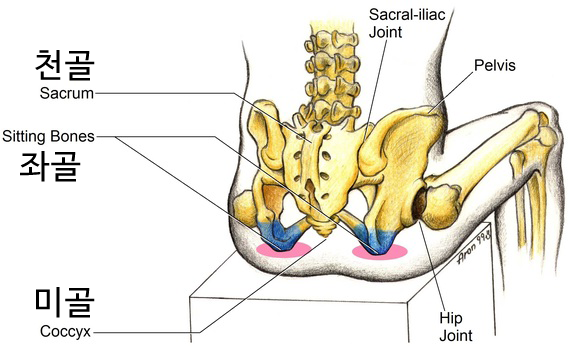
\includegraphics[width=\textwidth]{figures/sit.png}
             \caption{앉을 때의 좌골뼈의 위치}
             \label{fig:sit}
         \end{subfigure}
         \hfill
         \begin{subfigure}[b]{0.3\textwidth}
             \centering
             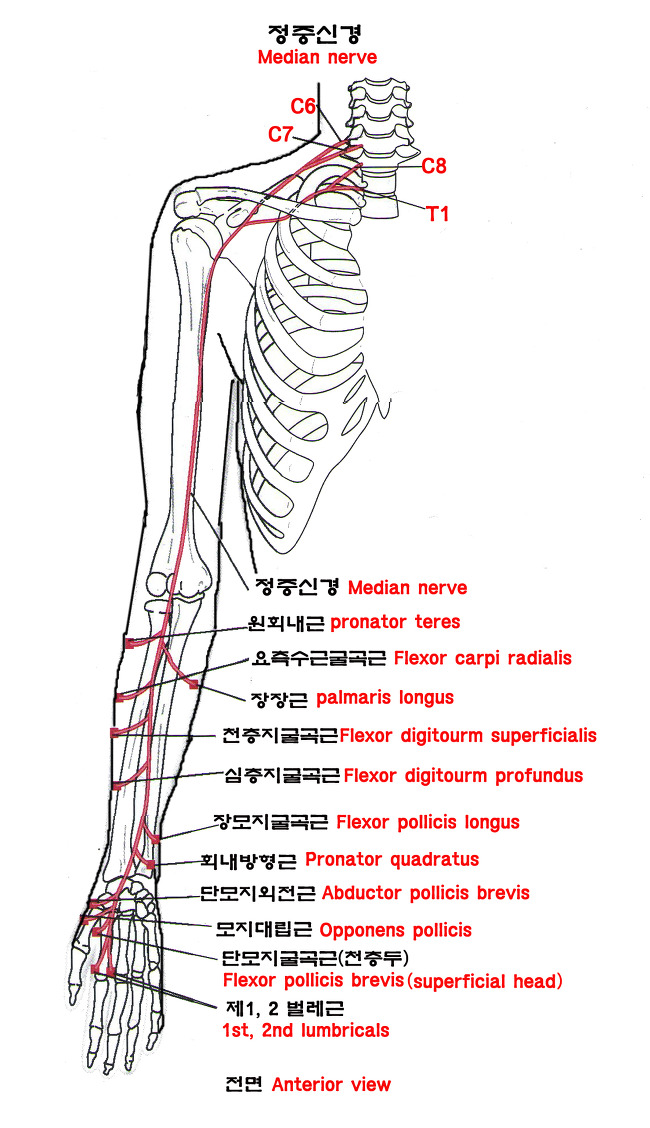
\includegraphics[width=\textwidth]{figures/med_nerve.jpg}
             \caption{정중신경이 지나는 모식도}
             \label{fig:1-b}
         \end{subfigure}
         \hfill
         \begin{subfigure}[b]{0.3\textwidth}
             \centering
             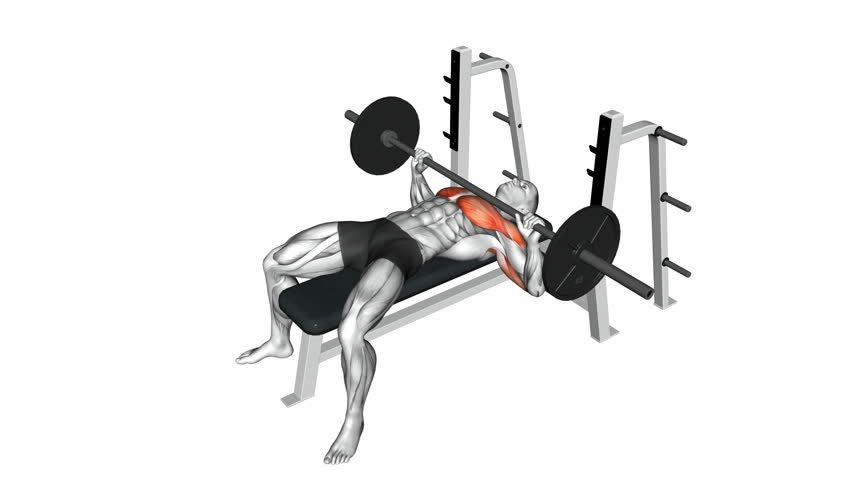
\includegraphics[width=\textwidth]{figures/bench.jpg}
             \caption{벤치프레스 자세}
             \label{fig:1-c}
         \end{subfigure}
            \caption{자세에 관한 이미지 자료}
            \label{fig:impl1}
    \end{figure}

몸의 맨 위쪽부터 알아보자. 눈높이는 모니터의 맨 위쪽 선에 맞추자. 턱은 당기고, 목은 펴주고, 어깨가 들리지 않게 의자의 높이 또는 책상의 높이를 조절해야 한다. 이 때, 어께의 좌우벨런스가 틀어지지 않도록(측만증) 주의하자. 가슴은 펴고, 등은 의자 등받이에 전체적으로 닿게 기대주자. 정중신경의 모식도를 보면 알겠지만, 어께가 앞으로 굽게 되면 해당 신경이 눌리면서 터널증후군을 유발하므로 유의하자. 팔은 팔꿈치 위쪽은 상체와 평행하게 두되 몸통과 팔 사이의 각도를 크게 해서 팔 에이밍시 어께가 돌지 않도록 한다. 팔꿈치를 몸통에 붙이고 팔에임하면 어께가 돌아가는 게 느껴짐. \footnote{꼭 완전히 평행할 필요는 없다! 그러나 팔이 너무 앞으로 나가서-이 경우 어께-팔꿈치 부분과 몸통과의 각도가 30도 이상으로 커지면 신경 눌려 통증 생김 라운드숄더가 되거나 힘줄이 당겨지지 않도록 주의하자.}, 팔꿈치 아래는 마우스패드와 수직하게 마우스패드에 살짝 올려준다. 이 때 회전축이 되는 손목과 팔꿈치의 특정 위치에 무게를 싣게 되면 통증을 유발하니, 패드에 살짝 대준다는 느낌으로 축을 설정해야 한다. 게다가 축을 세게 누르면 에임범위를 벗어나는 대상에 에이밍하거나 상하에임 시 축이 드드득거리면서 부드러운 에이밍이 불가능해진다. 이를 요약하면, 마우스를 들고 움직이는 게 아니라 친다고 생각하면 좋다.
허벅지는 의자에 닿도록, 양 발은 바닥을 지지해야 한다. 이때 발이 바닥에 닿지 않으면 발받침대를 구해서 사용하자. 발이 제대로 지지가 안 되면 무게중심이 앞으로 가면서 팔과 손목에 체중이 가해지니 주의해야 한다. 즉 몸 전체의 무게중심을 고르게 해야 패드 위에 올라간 부위의 무게중심도 고르게 분포된다. 등받이에 등이 전체적으로 닿는 것도 같은 맥락에서 중요하다. \footnote{어릴 때 의자에 엉덩이 끝까지 붙이고 앉으라고 했던 말이 사실 팔도 아프고 손목도 시큰거리게 되니까 했던 게 아닐까?} 이상으로 정리한 자세는 상체의 모양은 벤치프레스 자세와 유사하고, 어깨 아래 부분은 손걸레질 하는 자세랑 유사하다. 
이제 바르게 앉은 상태에서 팔을 편안하게 책상 위에 올려놓자. 어께와 팔의 모든 부분에 긴장이 풀리도록 해보자. 그게 당신의 에이밍 자세이다.

\section{근육과 축}
손을 움직이려면 전완근의 수축과 이완이 필요하고, 팔을 움직이려면 대흉근과 삼각근의 수축과 이완이 필요하다. from bardoz


\section{사운드플레이, crosshair replacement, peek}
에임의 상황을 화면과 조준선(화면의 중앙) 기준으로 에임의 상황을 나누어 보자. 상대가 내 화면(순간 에임범위 이내) 안에 있는지 여부와 조준선 위에 있는지 여부라는 기준으로 3가지 상황으로 나누어진다. 상대가 내 화면 밖에 있는 경우에는 상대가 발사하는 총알의 궤적, 사운드 등을 이용해 상대의 위치와 동선을 예측해서 헤드라인 근처에 에임을 대고 나가야 한다. 이를 peek이라고 부른다.
상대가  내 화면 안에 있는 경우, 상대를 조준선 위에 얹고 따라가면 된다. 상대가 내 크로스헤어 위에 있는 경우, 트레킹만 하면 된다.
에임범위 밖의 대상을 에이밍한 뒤에는 마우스를 들어서 팔과 손목을 다시 편한 위치로 옮겨주자. 이를 crossehair replacement라고 한다.

\section{키보드 에이밍}
오버워치는 움직임에 따른 반동이 없는 게임이기 때문에 키보드의 움직임을 에임에 활용할 수 있다.  캐릭터간 이동속도는 거의 동일하므로, 서로 좌우무빙을 치면서 교전중일 때, 나는 상대 몸 위에 크로스헤어를 올려둔 상태라면 상대가 나와 같은 방향으로 움직이면 에임을 위아래로만 움직이면서 쏘면 다 맞출 수 있다. 좌우 방향으로 상대속도가 0이기 때문이다. 상대가 나와 반대 방향으로 움직이면, 내가 가만히 서서 쏠 때보다 2배 빠른 속도로 마우스를 움직여야 한다. 이 경우 내 에임범위를 금새 벗어나게 되므로, 축을 풀어주지 않으면 트레킹이 끊기게 된다. 무빙을 적당히 섞을 경우 에임범위 문제를 어느 정도 해결할 수 있다. 
\subsection{위도우의 점프샷}
\footnote{https://youtu.be/T-sucESdZPQ}
\begin{enumerate}
    \item 상대가 있을 위치에 에임 미리 대기
    \item 줌부터 누르고 점프 후 방향키(차징을 위함)
    \item 벽이 좁으면 제자리에서 점프 후 줌 누르고 방향키
    \item 최종 위치는 상대의 위치와 벽 경계선을 일자로 둔다.
\end{enumerate}
\subsection{위도우의 훅샷}

\section{정보처리}
\subsection{상대가 주요시야범위 밖에 있을 경우}
사운드, 총알궤적으로 상대 케릭터의 헤드라인을 미리 잡아둔다.
\subsection{상대가 주요시야범위 안에 있을 경우}
\subsubsection{상대의 움직임 경로와 내 움직임 경로는 어떻게 하지}
\subsubsection{상대가 내 크로스헤어 밖에 있을 경우}
\begin{enumerate}
    \item 상대의 이동방향과 내 크로스헤어의 이동방향이 같은 경우
    \item 상대의 이동방향과 내 크로스헤어의 이동방향이 반대인 경우
\end{enumerate}
\subsubsection{상대가 내 크로스헤어 안에 있을 경우}
에이밍할 때는 목표지점과 목표가 움직이는 방향을 봐야 한다. 크로스헤어는 주변시아로 확인하며 크로스헤어를 상대 위에 올려놓기 위해 목표지점과 화면 중앙 사이의 거리를 계산하는 용도로 사용한다.
상대의 무빙을 예측하는 건 사람의 반응속도 한계 때문에 큰 도움이 안 된다. 예측은 상대의 동선을 생각하는 데에 사용하고, 캐릭터가 움직이는 방향에 따라 모양이 달라지는 점을 이용해서 무빙을 보고 쏘도록 하자. 예를 들어 루시우의 경우
    \begin{figure}[htp]
         \centering
         \begin{subfigure}[b]{0.3\textwidth}
             \centering
             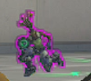
\includegraphics[width=\textwidth]{figures/read_moving/left.png}
             \caption{왼쪽으로 움직이는 경우}
             \label{fig:1-a}
         \end{subfigure}
         \hfill
         \begin{subfigure}[b]{0.3\textwidth}
             \centering
             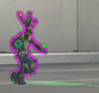
\includegraphics[width=\textwidth]{figures/read_moving/l2r.png}
             \caption{왼$\rightarrow$오의 뱡향전환}
             \label{fig:1-b}
         \end{subfigure}
         \hfill
         \begin{subfigure}[b]{0.3\textwidth}
             \centering
             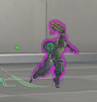
\includegraphics[width=\textwidth]{figures/read_moving/right.png}
             \caption{오른쪽으로 움직이는 경우}
             \label{fig:1-c}
         \end{subfigure}
            \caption{루시우의 움직임}
            \label{fig:read_moving}
    \end{figure}
와 같이 움직임에 따라 모양이 달라지고, 이는 에이밍에 활용할 만한 정보이다. //
연습 방법은 다음과 같다.
\begin{enumerate}
    \item ctrl+z를 눌러 UI를 끈다.
    \item 이 상태에서 상대의 움직임을 파악한 뒤 마우스로 이를 따라간다.
    \item 움직임 관찰 단계의 문제인지, 운동수행능력의 문제인지 파악한다.-방향전환은 속도가 느려지므로 더 디테일한 축을 활용해야함
    \item 문제를 해결한 뒤 2번으로 돌아간다.
\end{enumerate}
%FPS에서의 에임은 구면좌표계 위를 움직이게 된다. 하지만 내가 보고 있는 화면은 평면이므로, 그냥 상대를 바탕화면에 놓인 아이콘이라고 생각하고 클릭하자고 생각하면 도움이 될...수도 있다.

\section{상대의 움직임 경로, 범위}
상대의 주의력 자원에 대해서 생각해보자. 상대가 나를 의식하지 못할 때 쏘는 게 좋다.\footnote{볼트 포커싱이 강력한 이유} 무빙치는 적은 상대하기 까다롭다. 상대의 움직임 경로와 범위를 생각하면서 에임하면 쉽다. 예를 들어 리스폰에서 갓 나온 적은 직선으로 움직인다거나, 겐지의 이단점프는 높이 최대값이 어느정도 정해져있다는 점 등이다.


\section{감도}
감도는 자주 바꾸지 말고 하나 정해서 움직임을 훈련한다. 오버워치의 경우, 상대가 매우 빠르게 움직이므로 좌우로 180도는 커버할 수 있는 감도가 좋고, 이 감도는 보통 edpi 4000 언저리의 중감도이다.\footnote{필자는 800dpi 4.5, zoom-sens 30}

\section{힘조절}
일단 에임의 기초가 없는 사람들은 힘을 쭉 풀어주고 연습하자. 에이밍할 때 작용하는 힘은 마우스를 마우스패드에 수직한 방향으로 누르는 힘과 마우스를 미는 힘 두 가지가 있다. 상대가 크로스헤어를 기준으로 멀리 있거나, 빠르게 움직인다면 누르는 힘을 줄이고 미는 힘을 늘려야 하고, 가까이 있거나 느리게 움직이면 누르는 힘을 키우고 미는 힘을 늘려야 한다. 이 때 누르는 힘을 가했다가 다시 풀어주는 것이 중요한데, 자세가 잘못되어 무게중심이 엉덩이가 아니라 손과 팔로 옮겨지게 되면 누르는 힘을 다시 풀기 어려워져 에임이 점점 안 맞기 시작하니 주의하자. 마우스를 미는 힘은 다시 상하로 미는 힘과 좌우로 미는 힘으로 구분할 수 있는데, 상하에임의 경우 어께를 축으로 팔 전체를 위아래로 옮기거나 손가락으로 마우스를 위아래로 옮기는 방법이 있고, 좌우로 미는 힘의 경우 팔을 축으로 미는 힘과 손목을 축으로 미는 힘, 마우스를 축으로 손가락으로 미는 힘 세 가지가 있다. 이제 이 미는 힘과 누르는 힘을 연습해보자. AIMLAB은 STEAM에서 무료다!

\section{축}
안정감 있게 에임해야 할 때는 신체부위 한 곳을 지지대삼아서 트래킹하거나 끌어치기하면 안정감이 더해진다. 예를 들어 손목을 대고 손인사하듯 좌우로 까딱거리면 헤드라인 끌어치기가 쉽다. 이렇게 에이밍의 안정성을 위해 축을 설정하고 풀 수 있어야 한다. 이 때 주의할 점이 몇 가지 있다. 팔에임과 손목에임을 구분하여 팔 끝까지 쓴 후 손목을 움직이는 게 아니라 모든 관절을 섞어쓸 수 있어야 에임이 부드러워진다. 축을 설정할 때 팔꿈치부터 손목까지의 무게중심은 고르게 설정되어야 한다. 그렇지 않으면 상하에임 도중 손목이 들리면서 충격을 줄 수 있기 때문이다. 셋째로, 손목과 팔이 편하게 가동되는 범위까지만 움직여야 하고 그 이상은 사용하지 않아야 한다.

\section{마우스 그립}
마우스 그립법은 마우스 위에 손을 올려놓는 방법을 의미한다. 이 방법에는 여러 가지가 있으며 마우스의 모양과 유저의 신체조건에 따라 달라진다.
마우스 그립에 따라서 손목의 가동범위, 힘줄 및 신경에 주는 압력, 팔의 외회전 정도 등의 많은 요소가 달라진다. 가장 유명한 그립법은 팜, 클로, 핑거팁의 세 가지 그립법이지만 131 그립과 같이 손목을 중립에 두어서 가동범위의 대칭성을 맞춰주는 방법 등 다양한 그립법이 존재한다. 마우스 쉘의 모양과 무게 분포 및 유저 개개인의 손 크기 등 신체조건에 따라 마우스 그립을 다르게 해야 손목건강과 안정적인 에임을 유지할 수 있다.
- figure 추가할 것
마우스 양옆을 강하게, 윗면은 힘 빼야함 연필 잡는 것과 동일하게 생각, 단 중지와 검지가 컨트롤에 활용됨


\section{에임범위}
마우스를 옮기는 직접적인 신체부위는 팔꿈치와 손목, 손가락이다. 손끝에 가까운 부위를 사용할수록 한 번에 옮길 수 있는 범위가 좁아지지만 정밀한 마우스 컨트롤이 가능하고, 손끝에서 먼 부위를 사용할 수록 한 번에 옮길 수 있는 범위가 커지지만 정밀한 마우스 컨트롤이 어렵다. 또한, 일반적으로 신체구조상 왼쪽으로의 에임범위가 오른쪽으로의 에임범위보다 좁으므로 연습할 때 이를 고려해야 한다. 에이밍을 연습하기 전에, 바르게 앉은 상태에서 본인의 관절에 무리를 주지 않는 선에서의 각 부위별 에임 범위를 파악하고 있어야 한다.\\
 팔꿈치쪽 축으로부터 마우스 센서까지의 거리를 l,  손목쪽 축으로부터 마우스 센서까지의 거리를 r이라고 하자. l이 시작상태에서 움직인 각도를 $\theta$, r이 시작상태에서 움직인 각도를 $\alpha$ 라고 하면(당연히 단위는 radian), 마우스가 호를 따라 총 움직인 거리는 $l\theta+r\alpha$ 로 구할 수 있다. 이 때 마우스를 좌우로 움직이려면 직선으로 움직여야 하는데 각도가 너무 크면 직선이 아니라 곡선으로 움직이게 됨을 유의하자. 이를 막기 위해서는 축을 기준으로 팔과 손목을 까딱거린다고 생각하기보다는 마우스의 움직임에 집중하면 좋다.




\section{셀프 피드백 : 문제 판단 후 해결}
어느 정도 기초가 잡혔다면, 에이밍을 하면서 왜 안 맞는지 고민해서 수정할 수 있어야 한다. 대표적인 경우로 상대 몸 위에 크로스헤어를 올려놓지 못했는데 상대의 동선을 마우스로 따라가고 있는 상황이 있다. 이 경우에 상대의 위치가 내 에임범위 이내라면 끌어치기를 살짝 섞어서 크로스헤어를 올려놓고 트레킹하면 되고, 상대의 위치가 내 팔꿈치의 가동범위 밖이라면 팔꿈치 근처의 축을 풀고 팔을 전체적으로 이동시켜서 에이밍하거나, crosshair replacement 한 뒤 에이밍하면 된다. 이처럼 본인이 왜 안 맞는지 생각해보고 의식적으로 수정한 에이밍 방법이 무의식적으로 굳어진 습관을 이길 때까지 연습해보자. 연습은 마우스를 습관대로 까딱까딱거리는게 아니라 더 좋은 방법을 생각하고 무의식적으로 굳어진 습관을 의식적으로 덮어씌우는 과정이라는 걸 잊지 말자. 그리고 이론에 너무 매몰되지는 말자. 이 장의 목적은 건강하게, 잘, 게임하는 것이다!